% !TEX root = ../main.tex
%ex15_fig3.tex
%couronne de taille 10

\begin{figure}[h]
	\begin{center}
		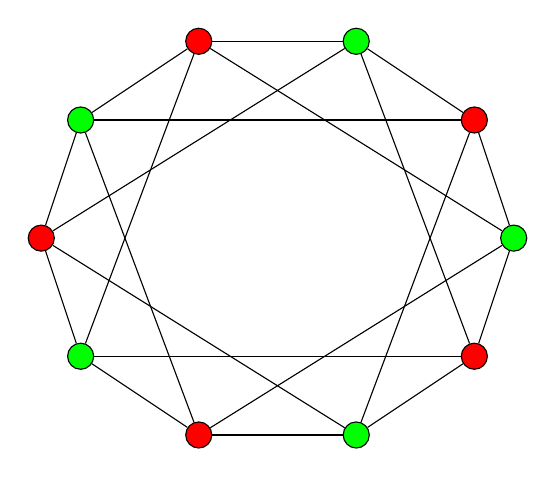
\begin{tikzpicture}
			\tikzset{node/.style={circle, draw=black}};
			\node[node,fill=red] (A) at (2,0) {};
			\node[node,fill=green] (B) at (4,0) {};
			\node[node,fill=green] (C) at (0.5,1) {};
			\node[node,fill=red] (D) at (5.5,1) {};
			\node[node,fill=red] (E) at (0,2.5) {};
			\node[node,fill=green] (F) at (6,2.5) {};
			\node[node,fill=green] (G) at (0.5,4) {};
			\node[node,fill=red] (H) at (5.5,4) {};
			\node[node,fill=red] (I) at (2,5) {};
			\node[node,fill=green] (J) at (4,5) {};

			\draw[black] (A) -- (B);
			\draw[black] (B) -- (D);
			\draw[black] (A) -- (C);
			\draw[black] (C) -- (E);
			\draw[black] (D) -- (F);
			\draw[black] (E) -- (G);
			\draw[black] (F) -- (H);
			\draw[black] (G) -- (I);
			\draw[black] (H) -- (J);
			\draw[black] (I) -- (J);
			
			\draw[black] (A) -- (G);
			\draw[black] (A) -- (F);
			\draw[black] (B) -- (H);
			\draw[black] (B) -- (E);
			\draw[black] (C) -- (D);
			\draw[black] (C) -- (I);
			\draw[black] (D) -- (J);
			\draw[black] (E) -- (J);
			\draw[black] (F) -- (I);
			\draw[black] (G) -- (H);
		\end{tikzpicture}
	\end{center}
	\caption{}
\end{figure}


